% Proprioception-grounded object recovery for learning from demonstration.
%
% Standalone figure source. Compile from the repo root with:
%     pdflatex -output-directory=figures Docs/fig_pipeline_tikz.tex
% which writes figures/fig_pipeline_tikz.pdf.
%
% To drop into Docs/twente-paper.tex as a full width figure:
%     \begin{figure*}[t]
%       \centering
%       \includegraphics[width=\textwidth]{figures/fig_pipeline_tikz.pdf}
%       \caption{...}
%       \label{fig:pipeline}
%     \end{figure*}
%
% Design intent. The figure carries two claims and nothing else:
%   1. Proprioception supplies the selection signal that vision cannot, so the
%      orange rail feeds "when" and "which role" while the blue rail only ever
%      supplies pixels. Stage 1 never sees an image.
%   2. The module's output is the object set O, not the policy F. Everything
%      outside our scope is drawn grey, and the unsolved generalization stage
%      is drawn dashed.
%
% Layout note. Stage pitch is 4.0 cm against a 2.3 cm box width, leaving a
% 1.7 cm channel for each edge label, which is set at text width 15 mm. Do not
% widen the boxes or shrink the pitch without shortening the edge labels, or
% they collide with the box borders.

\documentclass[tikz,border=6pt]{standalone}

\usepackage{mathptmx}
\usepackage{amsmath}
\usepackage{amssymb}
\usepackage{xcolor}

\usetikzlibrary{arrows.meta,positioning,calc,fit,backgrounds,shapes.geometric}

% ---------------------------------------------------------------- palette ---
\definecolor{cPropFill}{RGB}{253,236,212}
\definecolor{cPropLine}{RGB}{186,105,20}
\definecolor{cExtrFill}{RGB}{219,233,247}
\definecolor{cExtrLine}{RGB}{28,86,146}
\definecolor{cStageFill}{RGB}{227,242,230}
\definecolor{cStageLine}{RGB}{42,114,61}
\definecolor{cOutFill}{RGB}{235,225,246}
\definecolor{cOutLine}{RGB}{101,60,155}
\definecolor{cGreyFill}{RGB}{242,242,242}
\definecolor{cGreyLine}{RGB}{145,145,145}
\definecolor{cFutFill}{RGB}{253,248,222}
\definecolor{cFutLine}{RGB}{146,120,18}
\definecolor{cNote}{RGB}{168,38,38}

\begin{document}
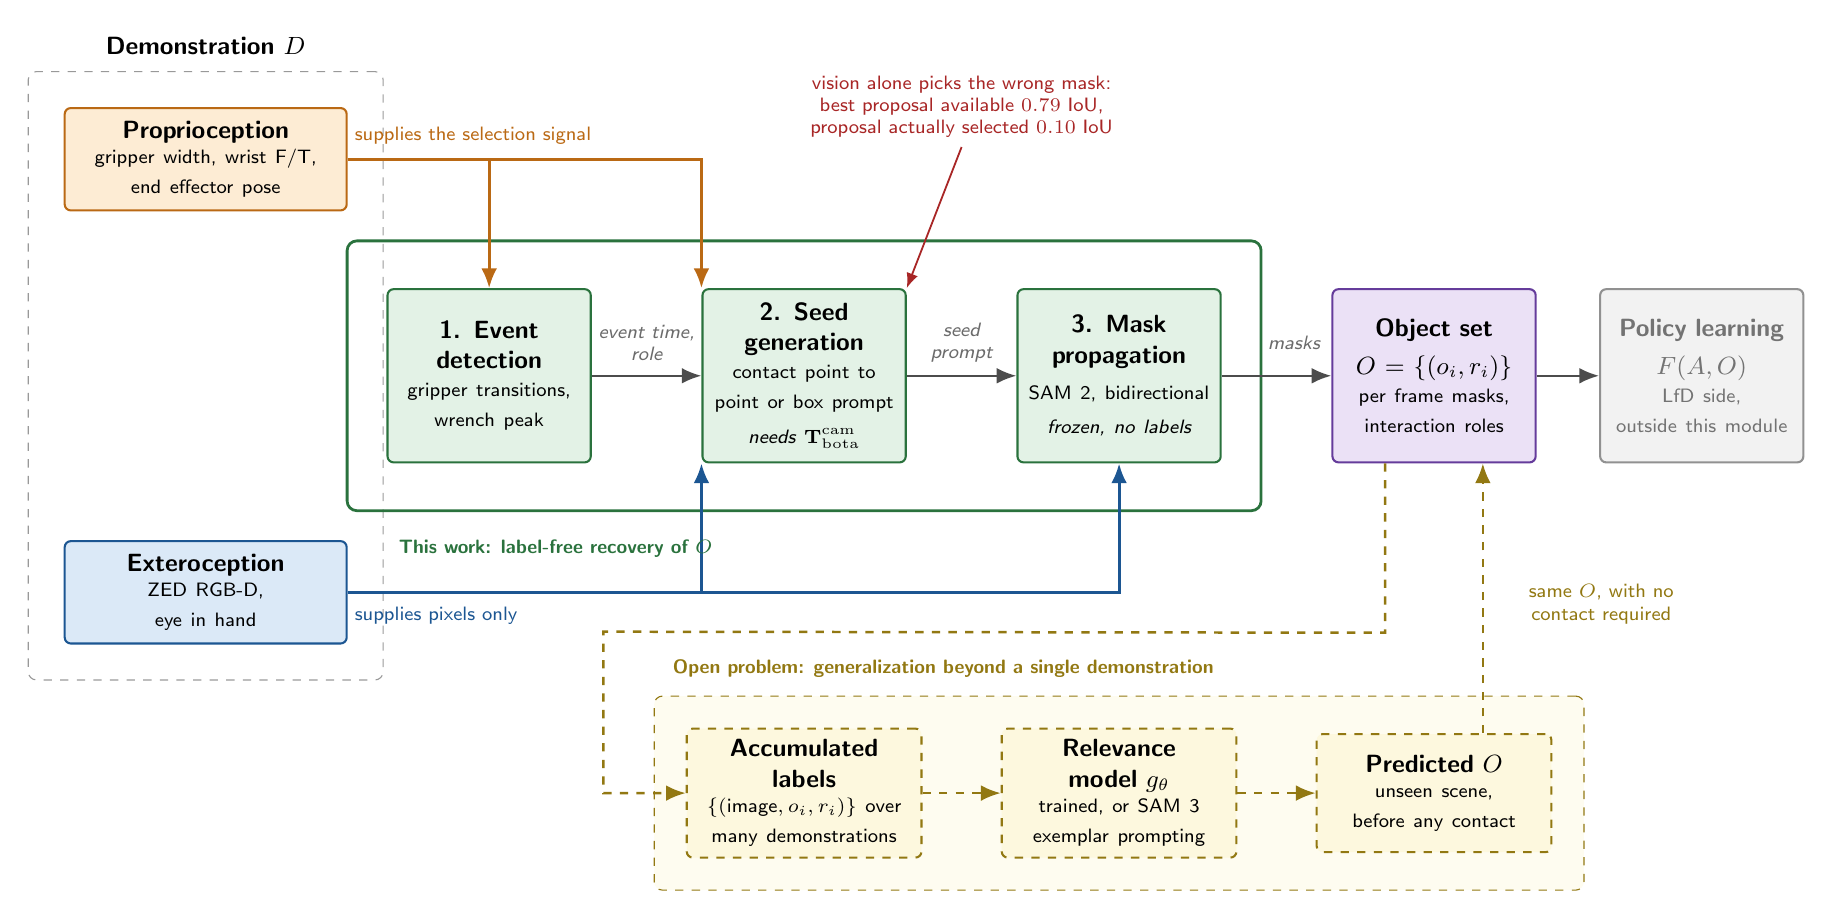
\begin{tikzpicture}[
  font=\sffamily,
  base/.style={
    draw, rounded corners=2.2pt, align=center,
    line width=0.75pt, inner sep=4pt, font=\sffamily\small},
  sensor/.style={base, text width=33mm, minimum height=13mm},
  prop/.style={sensor, fill=cPropFill, draw=cPropLine},
  extr/.style={sensor, fill=cExtrFill, draw=cExtrLine},
  stage/.style={base, fill=cStageFill, draw=cStageLine,
                text width=23mm, minimum height=22mm},
  outb/.style={base, fill=cOutFill, draw=cOutLine,
               text width=23mm, minimum height=22mm},
  greyb/.style={base, fill=cGreyFill, draw=cGreyLine, text=black!55,
                text width=23mm, minimum height=22mm},
  futb/.style={base, fill=cFutFill, draw=cFutLine, dashed,
               text width=27mm, minimum height=15mm},
  flow/.style={-{Latex[length=2.5mm,width=2.0mm]}, line width=0.9pt,
               draw=black!70},
  pflow/.style={flow, draw=cPropLine, line width=1.05pt},
  eflow/.style={flow, draw=cExtrLine, line width=1.05pt},
  fflow/.style={flow, draw=cFutLine, dashed, line width=0.9pt},
  % edge labels sit in the 1.4 cm channel between boxes, never on the line
  elab/.style={font=\sffamily\scriptsize\itshape, align=center,
               text=black!58, text width=15mm, inner sep=1pt},
  tag/.style={font=\sffamily\scriptsize, align=center, text=black!60},
  banner/.style={font=\sffamily\scriptsize\bfseries, align=left},
  note/.style={font=\sffamily\scriptsize, align=center, text=cNote},
]

% ------------------------------------------------------------- main lane ---
\node[stage] (evt)   at ( 4.15,0) {\textbf{1. Event}\\\textbf{detection}\\[2pt]
      {\scriptsize gripper transitions,\\ wrench peak}};
\node[stage] (seed)  at ( 8.15,0) {\textbf{2. Seed}\\\textbf{generation}\\[2pt]
      {\scriptsize contact point to\\ point or box prompt}\\[1.5pt]
      {\scriptsize\itshape needs $\mathbf{T}^{\mathrm{cam}}_{\mathrm{bota}}$}};
\node[stage] (track) at (12.15,0) {\textbf{3. Mask}\\\textbf{propagation}\\[2pt]
      {\scriptsize SAM 2, bidirectional}\\[1.5pt]
      {\scriptsize\itshape frozen, no labels}};
\node[outb]  (out)   at (16.15,0) {\textbf{Object set}\\[3pt]
      $O=\{(o_i,r_i)\}$\\[2pt]
      {\scriptsize per frame masks,\\ interaction roles}};
\node[greyb] (pol)   at (19.55,0) {\textbf{Policy learning}\\[3pt]
      $F(A,O)$\\[2pt]
      {\scriptsize LfD side,\\ outside this module}};

% --------------------------------------------------------------- sensors ---
\node[prop] (prop) at (0.55, 2.75) {\textbf{Proprioception}\\[1pt]
      {\scriptsize gripper width, wrist F/T,\\ end effector pose}};
\node[extr] (extr) at (0.55,-2.75) {\textbf{Exteroception}\\[1pt]
      {\scriptsize ZED RGB-D,\\ eye in hand}};

\begin{scope}[on background layer]
  \node[draw=black!40, dashed, rounded corners=3pt, inner sep=4.5mm,
        fit=(prop)(extr)] (dbox) {};
\end{scope}
\node[anchor=south, font=\sffamily\small\bfseries]
  at (0.55,3.96) {Demonstration $D$};

% ----------------------------------------------------------------- rails ---
\draw[pflow] (prop.east) -| (evt.north);
\draw[pflow] (prop.east) -| (seed.north west);
\draw[eflow] (extr.east) -| (seed.south west);
\draw[eflow] (extr.east) -| (track.south);

\node[tag, text=cPropLine, anchor=west] at (2.32, 3.05)
  {supplies the selection signal};
\node[tag, text=cExtrLine, anchor=west] at (2.32,-3.05)
  {supplies pixels only};

% ----------------------------------------------------- in lane data flow ---
\draw[flow] (evt)   -- (seed);
\draw[flow] (seed)  -- (track);
\draw[flow] (track) -- (out);
\draw[flow] (out)   -- (pol);

\node[elab] at ($(evt.east)!0.5!(seed.west)+(0,0.42)$)   {event time,\\ role};
\node[elab] at ($(seed.east)!0.5!(track.west)+(0,0.42)$) {seed\\ prompt};
% this channel is narrowed on the left by the scope box border at x = 13.80,
% so the label is single line and nudged right to clear it
\node[elab, text width=11mm]
  at ($(track.east)!0.5!(out.west)+(0.22,0.42)$)         {masks};

% ------------------------------------------------- the quantitative hook ---
\node[note, text width=39mm] (hook) at (10.15,3.42)
  {vision alone picks the wrong mask:\\
   best proposal available $0.79$ IoU,\\
   proposal actually selected $0.10$ IoU};
\draw[-{Latex[length=1.9mm,width=1.5mm]}, cNote, line width=0.65pt]
  (hook.south) -- (seed.north east);

% ------------------------------------------------------- open stage lane ---
\node[futb] (store) at ( 8.15,-5.30) {\textbf{Accumulated labels}\\[1pt]
      {\scriptsize $\{(\text{image},o_i,r_i)\}$ over\\ many demonstrations}};
\node[futb] (model) at (12.15,-5.30) {\textbf{Relevance model} $g_\theta$\\[1pt]
      {\scriptsize trained, or SAM 3\\ exemplar prompting}};
\node[futb] (pred)  at (16.15,-5.30) {\textbf{Predicted $O$}\\[1pt]
      {\scriptsize unseen scene,\\ before any contact}};

% return bus routed left of the open stage box entirely, so it never crosses
% the lane banner or the box border
\draw[fflow] ($(out.south)+(-0.62,0)$) -- ++(0,-2.15)
             -- (5.60,-3.25) -- (5.60,-5.30) -- (store.west);
\draw[fflow] (store) -- (model);
\draw[fflow] (model) -- (pred);
\draw[fflow] ($(pred.north)+(0.62,0)$) -- ($(out.south)+(0.62,0)$);

\node[tag, text=cFutLine, anchor=west, text width=24mm]
  at (16.95,-2.90) {same $O$, with no\\ contact required};

\begin{scope}[on background layer]
  \node[draw=cFutLine, dashed, rounded corners=3pt, inner sep=4mm,
        fill=cFutFill!45, fit=(store)(model)(pred)] (fbox) {};
\end{scope}
\node[banner, text=cFutLine, anchor=west]
  at ($(fbox.north west)+(1.2mm,3.4mm)$)
  {Open problem: generalization beyond a single demonstration};

% ------------------------------------------------------- scope separator ---
\begin{scope}[on background layer]
  \node[draw=cStageLine, rounded corners=3.5pt, line width=1.0pt,
        inner xsep=5mm, inner ysep=6mm, fit=(evt)(track)] (obox) {};
\end{scope}
% placed under the box: the top edge is crossed by the proprioceptive rail
% dropping into stage 1, and a banner there would sit on the line
\node[banner, text=cStageLine, anchor=west]
  at ($(obox.south west)+(5.5mm,-4.6mm)$)
  {This work: label-free recovery of $O$};

\end{tikzpicture}
\end{document}
